\chapter{Ankommen in München}

\section{Ummeldung -- Zweitwohnsitz}

Nach einem Umzug muss man sich in der neuen Stadt anmelden bzw. bei einem Stadtgebietswechsel ummelden. Entweder stattet man dazu dem KVR persönlich einen Besuch ab oder schickt das unterschriebene Formular per Post. Das Formular sowie nähere Infos zu den zuständigen Stellen finden sich im Internet im Dienstleistungsfinder auf den Seiten der Stadt München.

Benötigte Unterlagen für die Ummeldung: %Als Liste, damit man alles auf einen Blick hat.
\begin{itemize}
	\item Personalausweis oder Reisepass
	\item bei mehreren Wohnungen: Das Beiblatt für mehrere Wohnungen
	\item bei der Anmeldung per Post: Ausgefülltes Formular und Kopie des Personalausweises.
\end{itemize}

Sollte man sich dafür entscheiden, München oder seine bisherige Wohnung als Zweitwohnsitz anzumelden, fallen extra Steuern an. Die Zweitwohnsitzsteuer liegt bei 9~\% der jährlichen Nettokaltmiete. Können Einkünfte unter 25.000~€ nachgewiesen werden, so ist eine Befreiung von dieser Steuer möglich.

% Makros verwenden und ans ende!
\begin{urlList}
	\urlItem{http://muenchen.de/dienstleistungsfinder/muenchen/1063475/}
\end{urlList}

\section{Wohnen}
Wohnungen in München sind teuer, schwer zu bekommen und hart umkämpft. Die Mietpreise liegen
auch für Studenten ca. 50--100~€ über dem üblichen mittleren Preis in
Restdeutschland. Das Studentenwerk bietet auf seiner Homepage eine
gute Übersicht über alle Möglichkeiten des Wohnens:

\begin{itemize}
\item Studentenwerkswohnheime \ref{heim} sind 
	günstig aber schwer zu bekommen (erkundigt euch in den Verwaltungstellen direkt)
\item private Wohnheime, oft in eigener oder karitativer Trägerschaft
  (Bewerbungen sind nötig, z. T. gibt es Bedingungen, der Versuch lohnt sich)
\item
  Privatzimmer \ref{privat}
  werden vom Studentenwerk und der Mitwohnzentrale vermittelt.
\item Wohnen gegen Hilfe für ältere Leute, die der helfenden Hand dafür
  Wohnraum stellen.
\item andere Angebote \ref{andere}
\item Notunterkünfte \ref{caritas} \ref{hilfe}, falls alles schiefgeht
\end{itemize}

\begin{urlList}
	\urlItem{http://www.studentenwerk-muenchen.de/wohnen/wohnanlagen-des-studentenwerks-muenchen/}[heim]
	\urlItem{http://www.studentenwerk-muenchen.de/wohnen/vermittlung-von-privatzimmern/}[privat]
	\urlItem{http://www.studentenwerk-muenchen.de/wohnen/weitere-wohnangebote}[andere]
	\urlItem{http://www.caritastoelz.de/Page010179.htm}[caritas]
	\urlItem{http://www.wohnhilfe-muenchen.de/jugendhilfe/die-jugendpension-jup.html}[hilfe]
\end{urlList}


\subsection*{Selbst mieten} 
Eine Wohnung selber zu mieten ist teuer, aufwändig und oft werden Provisionen fällig. Suchen
lohnt sich in den gängigen Online Portalen und auf der Immobilienseite der
Süddeutschen Zeitung, auch online. Meistens werden Bürgschaften oder andere
Sicherheiten verlangt.  Wer vorbereitet zur Besichtigung kommt, ist im Vorteil.


\newpage
\raggedcolumns
\begin{multicols}{2}
\subsection*{Wohngemeinschaften}
Eine freundliche E-Mail mit einer Vorstellung eurer selbst und warum ihr
in diese WG passt ist wichtig.

\begin{urlList}
   	\urlItem{http://wg-gesucht.de}
	\urlItem{http://studenten-wg.de}
\end{urlList}




%\section{Wohnung}
%\begin{itemize}
%	\item Die beliebtesten Portale für WGs: \url{wg-gesucht.de} und \url{studenten-wg.de} (Wenn ihr euch bewerbt, schreibt mehr als euren Namen und Telefonnummer.  Stellt euch persönlich vor, bringt Bier mit ;-)).
%	\item Wohnheim: \url{studentenwerk-muenchen.de/wohnen}
%	\item andere Angebote: \url{studentenwerk-muenchen.de/wohnen/weitere-wohnangebote}
%	\item Notunterkünfte: \url{www.caritastoelz.de/Page010179.htm}, \url{www.wohnhilfe-muenchen.de/jugendhilfe/die-jugendpension-jup.html}
%\end{itemize}

%\section{GEZ}
%\begin{itemize}
%	\item Nach der Ummeldung wirst du wahrscheinlich bald Post von der GEZ bekommen.
%	\item Befreiung möglich, wenn du BAföG bekommst (Antrag stellen)
%	\item Gebühren Radio, Computer: 5,76~€/Monat \\
%Gebühren Radio, Computer, Fernseher: 17,98~€/Monat
%        \item \url{gez.de}
%        \item http://www.lawblog.de/index.php/archives/2011/04/15/generelles-hausverbot-fr\newline -gez-mitarbeiter-mglich/
%\end{itemize}

\section{Rundfunkbeitrag}
Seit letztem Jahr gibt es einen neuen Rundfunkbeitrag. Man zahlt nun pro Haushalt und nicht mehr pro Gerät. Die Gebühren von 17,98~€ sind pro Monat zu zahlen. Eine Befreiung ist unter Umständen möglich, wenn man beispielsweise BAföG erhält.

% Makros verwenden!
\begin{urlList}
    \urlItem{http://rundfunkbeitrag.de}
\end{urlList}

\columnbreak
\begin{center}
	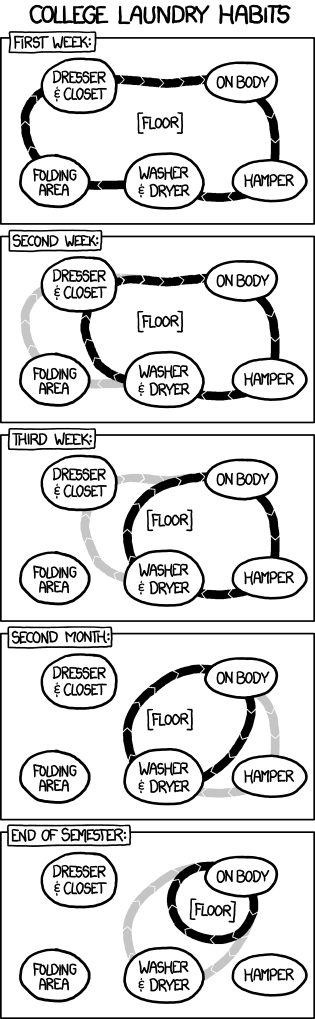
\includegraphics[width=0.9\linewidth]{comic_laundry}
\end{center}

\end{multicols}

\section{Mülltrennung}

Für die Restmüll- und Altpapiertrennung stehen in jedem Wohnblock eigene Tonnen zur Verfügung. Teilweise finden sich dort auch extra Biotonnen.
Die Container für Plastik, Dosen und Altglas sind über die Stadt verteilt und auch selten weit entfernt.
Sperrmüll, Elektroschrott und ähnliches sollte man am besten zu den Wertstoffhöfen bringen. Man sollte sich davor nach den Öffnungszeiten erkundigen. Im Gegensatz zu manch anderen Städten sind diese in München kostenlos.

% Makros verwenden!
\begin{urlList}
	\urlItem{http://awm-muenchen.de}
\end{urlList}

